%!TEX root = main.tex

\subsection{\textbf{RQ1:} Ho do software developers manage merge conflicts?}\label{RQ1}

\boldif{Results from interviews indicated that a common model of operating with merge conflicts exists.}
To understand the processes software developers use when working collaboratively on code, we asked interview participants to describe their current processes for handling merge conflicts.

\boldif{\textit{Add anecdotal quotes and descriptions from interviews to highlight these observations.}}
Several participants describe using tools that alert them to potential or current merge conflicts, processes for analyzing and understanding conflicting code prior to implementing a resolution, and the use of tools and checklists for validating that their resolution worked.
In the interview, P3 describes this process as:
\begin{quoting}
\textit{``Part of my job on the integration team requires that I check for bad regressions. I use scripts to track patches as they're being backported, so I know when and where to look if [a patch] introduces a conflict. [\ldots] And once I've fixed [the conflict], I try to compare with the previous version to make sure [the code] works in a similar way.''}
\end{quoting}
As described above, the user becomes aware of a merge conflicting by using these scripts, plans to resolve them by maintaining information about the locations of both the conflicts and patches, and evaluates the resulting patches to verify that the conflict has been resolved.
\boldif{Provide descriptions that link the stages of Merge Conflict model to this quote. Use it to drive description of simplified model description paragraph}

\boldif{Based on these anecdotal observations, we construct an initial model of the processes that developers employ when working with merge conflicts, see Fig.~\ref{model}.}
Our interview and survey results suggest that developers follow a series of phases through which they manage the lifecycle of individual merge conflicts.
To verify these phases, we construct a model of the Developer Processes for Merge Conflicts and examine each phase in detail in Section~\ref{results}.
Figure~\ref{model} provides an illustration of this model. 
It consists of four phases: \emph{awareness, planning, resolution,} and \emph{evaluation.}

\boldif{Discuss the fact that no other studies have shown that a model exists for merge conflicts}

\begin{figure}[!htbp]
\centering
\fbox{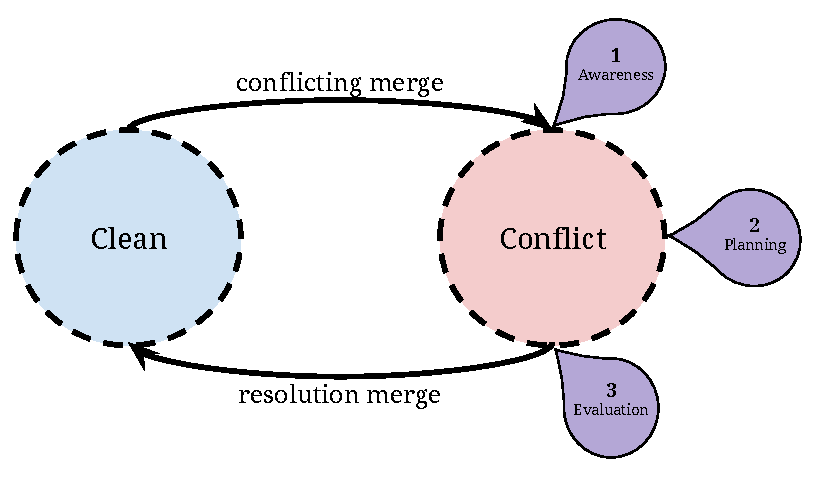
\includegraphics[width=0.90\textwidth,keepaspectratio]{imgs/MergeConflictModel}}
\caption{Model of Developer Processes for Merge Conflicts. Developers alternate between \textit{clean} and \textit{conflicting} states within their codebase. Beginning from (1)~\textit{development}, developers maintain (2)~\textit{awareness} of conflicts within the codebase in different ways. Once aware, developers begin (3)~\textit{planning} for a (4)~\textit{resolution} to fix the conflict. And finally, developers (5)~\textit{evaluate} the effectiveness of their deployed resolutions (returning to \emph{planning} if the resolution failed).\vspace*{-0.3\baselineskip}}
\label{model}
\end{figure}

\boldif{Awareness is how developers become aware}
The \emph{awareness} phase consists of the actions developers take to become aware of merge conflicts.
This could be accidental, or passive, as the developer will become aware of a merge conflict when attempting to merge changes or perform a pull.
At the other end of the spectrum are developers who \emph{proactively} monitor for merge conflicts as they write code.
They are actively looking for changes that might be problematic, either manually or through the use of specialized tools.

\boldif{Planning is when developers plan their future actions}
Secondly, the \emph{planning} phase occurs after the developer has become aware that a conflict has occurred, and they are about to tackle the conflict.
This includes the decision of when they will try and resolve the conflict.
Some developers might try and resolve it immediately, while others might postpone the resolution.
Some might change their strategy depending on the conflict, incoming deadlines, or availability of resources.
This also includes other actions, such as if they are going to tackle the conflict alone, or collaborate with other developers knowledgeable in the area of conflict.

\boldif{Resolution is the action of implementing a resolution. Mundane and well understood, so we focus on the other three.}
Third, the \emph{resolution} phase occurs once the developer has established a plan and has begun implementing it.
Prior work has primarily focused on this aspect of merge conflicts~\cite{nishimura,mens2002state,Brun2011}.
Therefore, we note that the resolution phase is important to the overall success of any merge conflict resolution, and focus on the other three phases in order to better understand the overall process.

\boldif{Evaluation is how developers check that their solution is correct}
Finally, after the conflict has been resolved, developers enter in the \emph{evaluation} phase.
In this phase, the developer has to evaluate their resolution before considering the conflict as resolved.
This is to ensure the correctness of the resulting code.
Possible actions during this stage includes compiling the source code.
Developers wanting more guarantees can go a step further and run the tests.
Finally, some groups have policies such as code reviews that need to be performed on the merge conflict resolution.
 
\boldif{To explore and validate this model, we asked developers to reflect upon how they become aware of merge conflicts, how they plan for merge conflict resolutions, and how they evaluate their resolutions in the \textit{Processes Survey}~(S1).}
In order to explore and validate this model, and our assumptions, we conducted the \emph{Processes Survey}~(S1).
We plan on understanding how developers become aware of merge conflicts (what steps they take, what tools they use, etc.).
We also want to investigate their strategies for dealing with merge conflicts and how they decide whether the resolution has addressed all their concerns.

\boldif{We present the results to these research questions in Sections~\ref{RQ1a}, \ref{RQ1b}, and \ref{RQ1c}.}
Sections~\ref{RQ1a}, \ref{RQ1b}, and \ref{RQ1c} presents the results to these research questions.

\subsubsection{\textbf{RQ1a:} How do software developers become \textbf{aware} of merge conflicts?}\label{RQ1a}
\vspace*{-0.5\baselineskip}
\begin{center}
\fbox{\parbox{\dimexpr\linewidth-5\fboxsep-2\fboxrule\relax}{\small\centering\raggedleft \textit{``It isn't that they cannot find the solution. It is that they cannot see the problem.''\\ -- G.K. Chesterton}}}%
\end{center}
\vspace*{+0.3\baselineskip}

\boldif{Developers use 2 methods for becoming aware of merge conflicts: proactive and reactive.}
From the \textit{Processes Survey}~(S1) we found that 29.41\% of participants do not actively monitor for merge conflicts during their development activities.
For the rest of the developers who answered with \emph{yes} or \emph{sometimes} (61.77\%), we identified 61 different tools mentioned in 126 instances.

\nsubsection{Reactive and Proactive Monitoring for Merge Conflicts}

\boldif{Reactive detection only notifies developers that a merge conflict \emph{has happened}. Developers use it to minimize the size/complexity of the conflict, or it's impact on the team.}
Reactive monitoring for merge conflicts will notify the developer that a conflict has already occurred.
However, developers still use this process to manage or reduce the complexity of a conflict.
For the developers that answered that they monitor for merge conflicts (replied either \emph{yes} or \emph{sometimes}), we found that 73.68\% (42 out of 57 responses; 4 respondents left this field blank) described reactive processes.
For example, one developer said they use integration tools to detect merge problems before they advance to testing:
\begin{quotation}
	[\ldots] integration tests tell us if builds are breaking and we use those to locate merge conflicts. [\ldots] we use it to catch merge bugs before they go to smoke testing for release
\end{quotation}
Another developer mentioned that they try to solve merge conflicts early in order to minimize disruptions to the team:
\begin{quotation}
	We try to catch conflicts early so that fewer developers have to be involved in looking at broken code.
\end{quotation}

\boldif{Proactive monitoring allows devs to detect MC before they happen. However, it is more involved, as it requires a lot more manual effort from the developers.}
Proactive monitoring allows developers to preemptively catch merge conflicts before they happen.
Some developers mentioned they achieved this by manually tracking incoming changes:
\begin{quotation}
	I monitor commit logs before I begin merging branches so that I see any potentially overlapping code that will break the merge.
\end{quotation}
Other teams rely more on communication.
This can happen during regular team meetings, to make sure that everybody is aware of each other's tasks:
\begin{quotation}
	[\ldots] standups allow us to know where everyone is working that week.
\end{quotation}
Others will broadcast their changes in order to notify team members if they will make breaking changes:
\begin{quotation}
	[\ldots] send emails before making breaking changes to the API or related sub-modules.
\end{quotation}

\nsubsection{Tools for Monitoring for Merge Conflicts}

\boldif{The tools that developers use allow for only a \emph{reactive} approach.}
Examining the tools used by respondents with reactive processes, we find that 87.72\% of our respondents rely on version control systems (e.g. Git, SVN, TFS, CVS), while 21.05\% use continuous integration systems (e.g. Jenkins, Travis CI, TeamCity).
Table~\ref{s1_toolset} presents the top 10 tools developers use when monitoring for merge conflicts.
It is worth noting that tools, such as those for continuous integration and developer notification systems (e.g. PagerDuty) are used only by developers relying on a \emph{reactive} strategy.
The majority of the tools developers use for merge conflict monitoring only allow a reactive approach to monitoring.

%\boldif{Devs do not use existing workspace awareness tools that come from the acadmemia.}
%When collaborating, developers generally rely on passive communication tools, like email, to coordinate.
%Developers are currently not leveraging the functionalities provided by many research prototypes (e.g., Palant\'{i}r~\cite{palantir}, Crystal~\cite{Brun2011}) that are specifically designed to facilitate proactive conflict detection.

\begin{table}[!htbp]
\renewcommand{\arraystretch}{1.3}
\caption{Merge Awareness Toolsets (Top 10) from Processes Survey (S1)}
\label{s1_toolset}
\centering
\begin{tabularx}{\textwidth}{ll|cc|c}
\toprule
% \textbf{Par.}\parnote{Par. = Total number of survey participants using each tool.}
% \vspace*{-0.3\baselineskip}
  \parnoteclear % tabularx will otherwise add each note thrice
  Tool\parnote{\textit{Processes Survey}~(S1) participants were allowed to provide multiple tools. 57 out of 102 respondents (56\%) indicated the use of at least one merge awareness tool.} & Description & Proactive\parnote{Participants using this tool with a proactive strategy.} & Reactive\parnote{Participants using this tool with reactive strategy.} & Par.\parnote{Par. = Total number of survey participants using each particular tool.}\\
\midrule
  Git & Version Control System & 10 & 30 & 40\\
  Email (unspecified) & Email Client or System & 2 & 4 & 6\\
  GitHub & Website & 2 & 5 & 7\\
  SVN & Version Control System & 0 & 4 & 4\\
  Visual Studio & IDE & 1 & 2 & 3\\
  PagerDuty & IT Incident Manag. Sys. & 0 & 3 & 3\\
  GitLab & Website & 2 & 1 & 3\\
  Jenkins & Continuous Integration & 0 & 3 & 3\\
  VCS (unspecified) & Version Control System & 2 & 2 & 4\\
  Team Foundation Server & Version Control System & 1 & 1 & 2\\
\bottomrule
\end{tabularx}
\parnotes
\end{table}

\begin{comment}
We asked the Processes Survey (S1) participants to categorize and describe their monitoring processes: whether and how they monitor for merge conflicts, and how they determine the urgency of any merge conflicts that occur.
We found that 32.26\% of participants do not monitor for merge conflicts during their development sessions.
For the 67.74\% participants that indicate \textit{yes} or \textit{sometimes} to the question of monitoring for merge conflicts, we asked them to describe the processes and tools that they use for monitoring.

We identified 61 different tools from the 126 instances.
Some mentioned generic responses such as \textit{``email''}, for which we create a separate category.
Table~\ref{s1_toolset} lists the top 10 most common tools used by participants to monitor for merge conflicts.

In examining the list of these tools, we note that developers most often use version control systems (e.g. Git, SVN, TFS, and unspecified VCS) to handle tracking changes, and potentially identifying merge conflicts, within a codebase.
In this list, there is also one continuous integration (CI) platform (Jenkins), an IT incident response platform (PagerDuty), and two VCS-hosting websites (GitHub and GitLab).
This indicates that developers are currently relying on reactive tools that indicate the presence of merge conflicts after they have been introduced to a codebase.

We then evaluate responses for processes that are proactive or reactive in nature (using card sorting and negotiated agreement).
We find that 42 of 57 responses (73.68\%) described reactive processes of merge conflict monitoring; such as waiting for build systems notifications, examining commit logs, or checking code consistency during branch integration.

Examining the tools used by respondents with reactive processes, we find that 64.28\% of our respondents use version control systems (Git, SVN, TFS, CVS), while 29.19\% use continuous integration systems (Jenkins, Travis CI, TeamCity).
We find that developers are currently not leveraging the functionalities provided by many research prototypes (e.g., Palant\'{i}r~\cite{palantir}, Crystal~\cite{Brun2011}) that are specifically designed to facilitate proactive conflict detection.

\begin{table}[!htbp]
\renewcommand{\arraystretch}{1.2}
\caption{Factors for Determining the Urgency of a Merge Conflict from Processes Survey (S1)}
\label{s1_conflict_urgency}
\centering
\begin{tabularx}{\textwidth}{c | l | c | r}
\toprule
  \parnoteclear % tabularx will otherwise add each note thrice
  Factor & Description & \# Participants\parnote{Each entry represents the number (and percentage) of participants that indicated that particular factor was relevant. 72 out of 102 respondents (71\%) provided their factors.} & Percentage (\%)\\
\midrule
  F1 & No systematic factors & 22 & 30.56\% \\
  F2 & External dependencies & 17 & 23.61\% \\
  F3 & Code under conflict & 17 & 23.61\% \\
  F4 & Project structure & 16 & 22.22\% \\
\bottomrule
\end{tabularx}
\parnotes
\end{table}

In addition, we identified \textbf{X} distinct categories of processes that developers use to monitor for merge conflicts (see Table~\ref{s1_monitoring_processes}).
\boldif{Provide further discussion on the results of Q7 analysis; analysis between Caius and Nick still needed to group the processes into groups}
\boldif{Provide results and discussion for Q8; factors for determining urgency of a merge conflict.}

\end{comment}

\subsubsection{\textbf{RQ1b:} How do software developers \textbf{plan} for merge conflict resolutions?}\label{RQ1b}
\vspace*{-0.5\baselineskip}
\begin{center}
\fbox{\parbox{\dimexpr\linewidth-5\fboxsep-2\fboxrule\relax}{\small\centering\raggedleft \textit{``If you are unable to understand the cause of a problem, it is impossible to solve it.''\\ -- Naoto Kan}}}%
\end{center}
\vspace*{+0.3\baselineskip}

\boldif{Developers use different strategies for dealing with MC}
When encountering a merge conflict, developers have different strategies at their disposal.
They can either: (a) defer the merge conflict for a later date, or; (b) solve the conflict.
In the \textit{Processes Survey}~(S1) we sought an understanding of these strategies and when developers use them.

\boldif{The first option is that they might defer the MC, for a later time}
The easiest option when encountering a merge conflict is to simply not deal with it.
Indeed, we found that 56.18\% of participants have deferred at least once when responding to a merge conflict.
The reasons for deferring are varied and include the \textit{complexity of the conflicting code} (D1), the \textit{number of conflicting code locations} (D2), and the \textit{ownership of the conflicting code} (D3) (additional reasons D4--D7 can be found in Table~\ref{s1_deferring_response}).
One of the participants succinctly describes how they consider the \emph{ownership of the conflicting code} when deciding whether to defer:
\begin{quotation}
	Code is mine? I fix it. Code is others? I submit PR or bug reports.
\end{quotation}
This indicates that the deferral is not always temporal, but can also be logistical when developers will defer to other team members.

\begin{table}[!htbp]
\renewcommand{\arraystretch}{1.2}
\caption{Factors in Deferring Responses to Merge Conflicts from Processes Survey (S1)}
\label{s1_deferring_response}
\centering
\begin{tabularx}{\textwidth}{>{\rowmac}c | >{\rowmac}l | >{\rowmac}c | >{\rowmac}r <{\clearrow}}
\toprule
  \parnoteclear % tabularx will otherwise add each note thrice
  Factor & Description & \# Selections\parnote{\textit{Processes Survey}~(S1) respondents were allowed to select multiple factors. 44 out of 102 respondents (43\%) selected more than one factor.\vspace*{-0.9\baselineskip}} & Percentage (\%)\textsuperscript{i} \\
\midrule
  D1 & Complexity of the conflicting code & 36 & 25.00\% \\
  D2 & Number of conflicting code locations & 32 & 22.22\% \\
  D3 & Ownership of the conflicting code & 25 & 17.36\% \\
  D4 & Size of the conflicting code & 20 & 13.89\% \\
  D5 & Approaching deadlines & 13 & 9.03\% \\
  D6 & Work schedule constraints & 2 & 1.39\% \\
  D7 & Other\hspace{4.6cm} & 7 & 4.86\% \\
\bottomrule
\end{tabularx}
\parnotes
\end{table}

\nsubsection{Deferring Response to Merge Conflicts}

\boldif{Deferring can have bad consequences, including increased complexity and delaying features. Organizations have sometimes changed the policy to prevent this.}
Deferring the merge conflict resolution comes with a price.
Table~\ref{effects-deferral} shows the top effects of deferring a response to a merge conflict.
The most common effect was that developers have had to stop the development (\emph{Stop the Presses,} 15 responses) in order to resolve the conflicts.
The second most common effect is the \textit{increased complexity} of the conflicts (E2), as it was reported by 9 of our participants.
One participant noted that:
\begin{quotation}
	Deferring a merge conflict simply kicks the can down the road (or off a cliff). Typically resolving the conflict only gets more difficult as time passes.
\end{quotation}
A respondent even hinted that the increased complexity can be quite severe, on an order of magnitude greater than if the conflict were addressed immediately:
\begin{quotation}
	Untangling takes days instead of minutes when it gets too out of hand.
\end{quotation}
In some cases, features had to be removed from releases, in order for integration problems to be mitigated and the conflict to be successfully resolved:
\begin{quotation}
	We have had several releases come up short in new features because they got delayed by integration problems.
\end{quotation}
Finally, in order to prevent similar problems arising, some organizations have instituted \textit{policy changes} (E4) to prevent this from happening in the future:
\begin{quotation}
	We've had devs push a bunch of code up before going on holiday and mucking up a release, so we've instituted an all hands on deck policy for the 2 weeks leading up to a major release
\end{quotation}

\boldif{However, some effect can be severe, including impact to customers, or having to reimplement features.}
In one extreme case, a participant reported that the effects of an unresolved merge conflict affected production software (E7), which resulted in downtime of the product, as it broke functionality:
\begin{quotation}
	Broke the app for customers until we could get a patch pushed [\ldots].
\end{quotation}
Finally, the merge conflicts can get too severe and intractable for developers to cope with the complexities.
In these types of situations, developers have to resort to the \emph{Nuclear Option} (E5), where they scrap their changes and reimplement them:
\begin{quotation}
	Uh.... KABOOM! More changes came in and everything piled up. Nothing to do but wipe it all back to clean and start trying to piece things back together.
\end{quotation}

\begin{table}[!htbp]
\renewcommand{\arraystretch}{1.2}
\caption{Effects of Deferring Response to a Merge Conflict from Processes Survey (S1)}
\label{effects-deferral}
\centering
\begin{tabularx}{\textwidth}{>{\rowmac}c | >{\rowmac}l | >{\rowmac}c | >{\rowmac}r <{\clearrow}}
\toprule
  \parnoteclear % tabularx will otherwise add each note thrice
  Effect & Description & \# Participants\parnote{46 out of 102 respondents (45.1\%) provided a description of the effects of deferring.\vspace*{-0.8\baselineskip}} & Percentage (\%)\textsuperscript{i} \\
\midrule
  E1 & Stop the Presses & 15 & 32.61\% \\
  E2 & Increased complexity & 9 & 19.57\% \\
  E3 & Non-operation effects & 5 & 10.87\% \\
  E4 & Policy/cultural changes & 3 & 6.52\% \\
  E5 & The Nuclear Option & 2 & 4.35\% \\
  E6 & Physical manifestations & 1 & 2.17\% \\
  E7 & Impact beyond the organization \hspace{1cm} & 2 & 2.17\% \\
\bottomrule
\end{tabularx}
\parnotes
\end{table}
\vspace{0.8em}

\nsubsection{Initial Strategies}

\boldif{If they have not deferred, they need to understand the (changes in the) conflict}
Other than deferring, the other remaining option for developers is to resolve the conflict.
They primarily approach merge conflicts by \textit{examining the merge} (U1), \textit{analyzing or manipulating the code} (U2), or \textit{examining the code} (U3).
Table~\ref{s1_understanding_code} lists all six strategies described by \textit{Processes Survey}~(S1) respondents.

\begin{table}[!htbp]
\renewcommand{\arraystretch}{1.2}
\caption{Initial Strategies for Understanding Conflicting Code from Processes Survey (S1)}
\label{s1_understanding_code}
\centering
\begin{tabularx}{\textwidth}{>{\rowmac}c | >{\rowmac}l | >{\rowmac}c | >{\rowmac}r <{\clearrow}}
\toprule
  \parnoteclear % tabularx will otherwise add each note thrice
  Strategy & Description & \# Participants\parnote{79 out of 102 respondents (77\%) provided a description of their initial strategy.\vspace*{-0.3\baselineskip}} & Percentage (\%)\textsuperscript{i} \\
\midrule
  U1 & Examining the merge & 26 & 32.91\% \\
  U2 & Analysis/manipulation of the code & 19 & 24.05\% \\
  U3 & Examining the code & 18 & 22.79\% \\
  U4 & Focus on design concerns & 8 & 10.13\% \\
  U5 & Examine project organization & 6 & 7.60\% \\
  U6 & No strategy\hspace{3.5cm} & 2 & 2.53\% \\
\bottomrule
\end{tabularx}
\parnotes
\end{table}
\vspace{0.8em}

\boldif{The most common strategies for understanding the conflict are examining the conflict and analysis/manipulation of the code.}
One participant described their strategy of examining the conflict as:
\begin{quotation}
	Reviewing the most recent commits (comments and code) to see whether it's a shallow conflict or not.
\end{quotation}
	Another participant indicated their strategy of analyzing the code involves:
\begin{quotation}
[\ldots] determining if the merge conflict involves important functionality; stepping through with a debugger helps.
\end{quotation}
Overall, we find that developers initially focus on the code involved in the merge conflict or information related to the merge itself.

\boldif{Surprisingly, some developers do not have a strategy for MCR}
Surprisingly, we found that two of our participants (2.53\% of respondents) indicated that they \textit{``don't have a strategy''} or \textit{``mostly try to fix it as soon as possible.''}

\begin{figure}[!htbp]
\centering
\fbox{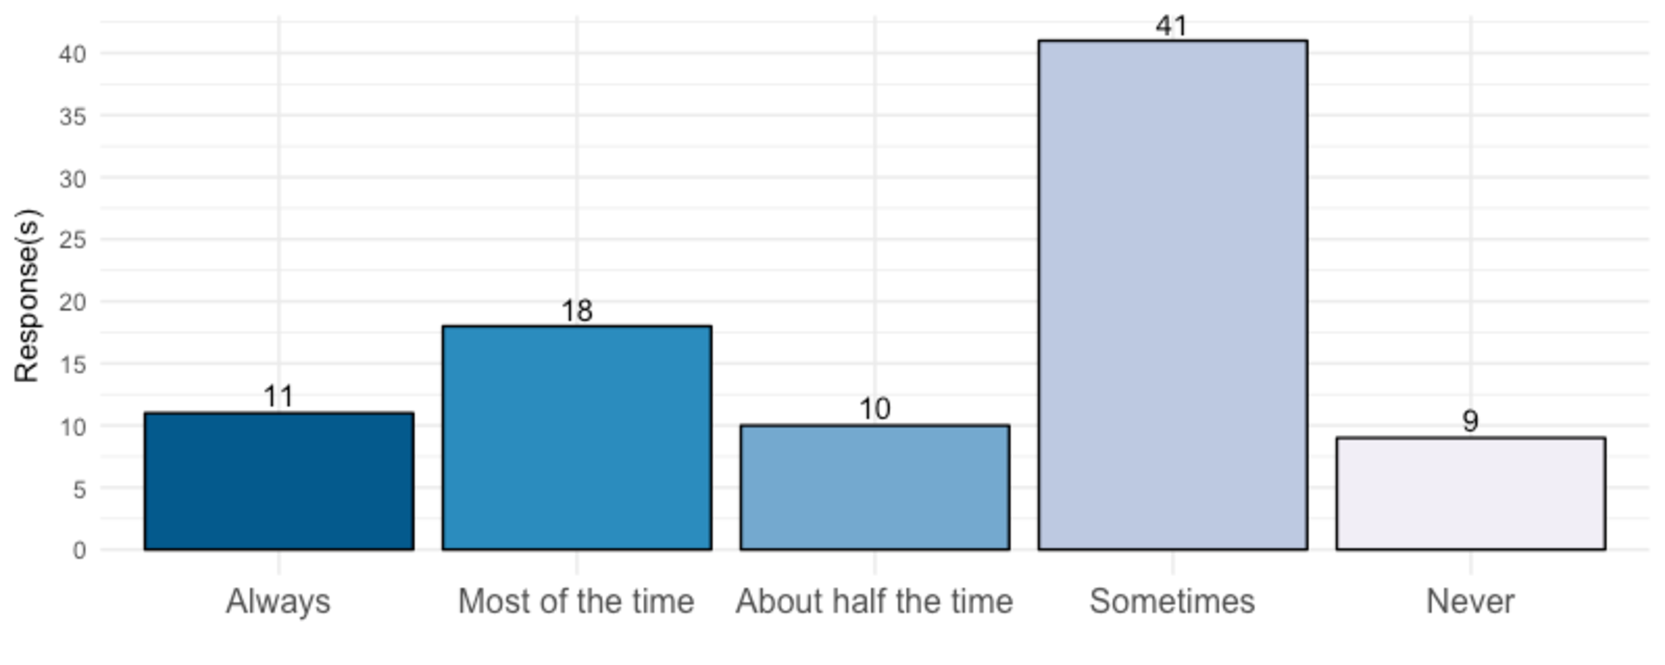
\includegraphics[width=0.98\textwidth,keepaspectratio]{imgs/CodeOwnershipFactor}}
\caption{Degree of Code Ownership as a Factor in Merge Conflict Strategies. Scale: 1 is \textit{Always} and 5 is \textit{Never}. 89 out of 102 respondents (87.26\%) provided a response to this question in the \textit{Processes Survey}~(S1).\vspace*{-0.3\baselineskip}}
\label{fig:code-ownership-resolution}
\end{figure}

\nsubsection{Code Ownership in Merge Conflict Resolution Strategies}

\boldif{The role of code ownership in the resolution strategy.}
Finally, we found that, on average, participants indicate that code ownership factors \textit{about half the time} in their strategy of code ownership (mean: $3.21$ on a 5-point Likert-type scale).
This is consistent with their responses for their criteria for deferring a resolution, where it is the third most common factor in their decision. 
Only 10.11\% of participants indicated that code ownership \textit{never} factors into their resolution strategy (see Figure~\ref{fig:code-ownership-resolution}).

\begin{comment}

Software developers adopt strategies for increasing their own efficiency and productivity.
We asked Process Survey (S1) participants a series of questions relating to their strategies for gaining understanding about a merge conflict, prioritizing merge conflict resolutions, and deferring resolutions when necessary.

\subsubsection{Initial Strategies for Understanding Conflicting Code}

We asked participants to describe their initial strategies for understanding conflicting code involved in a merge conflict.
We find that developers primarily approach merge conflicts by \textit{examining the conflict} (U1), \textit{analyzing or manipulating the code} (U2), or \textit{examining the code} (U3) (see Table~\ref{s1_understanding_code}).

One participant described their strategy of examining the conflict as:
\begin{quoting}
\textit{``Reviewing the most recent commits (comments and code) to see whether its a shallow conflict or not.''}
\end{quoting}
Another participant indicated their strategy of analyzing the code involves:
\begin{quoting}
\textit{``[\ldots] determining if the merge conflict involves important functionality; stepping through with a debugger helps.''}
\end{quoting}
Overall, we find that developers initially focus on the code involved in the merge conflict or information related to the conflict itself.
This illustrates the importance of code metrics and tool support for developers looking to gain understanding about a merge conflict when planning for a resolution.

Surprisingly, we found that two of our participants (2.53\% of respondents) indicated that they \textit{``don't have a strategy''} or \textit{``mostly try to fix it as soon as possible.''}
The existence of this \textit{no strategy} approach is anecdotal, but curious, since we assume that developers are rational actors seeking to organize themselves in ways that increase the likelihood of successful outcomes.
And yet this strategy appears to go counter to that notion.

\begin{table}[!htbp]
\renewcommand{\arraystretch}{1.2}
\caption{Initial Strategies for Understanding Conflicting Code from Processes Survey (S1)}
\label{s1_understanding_code}
\centering
\begin{tabularx}{\textwidth}{>{\rowmac}c | >{\rowmac}l | >{\rowmac}c | >{\rowmac}r <{\clearrow}}
\toprule
  \parnoteclear % tabularx will otherwise add each note thrice
  Category & Description & \# Participants\parnote{79 out of 102 respondents (77\%) provided a description of their initial strategy.} & Percentage (\%)\textsuperscript{i} \\
\midrule
  U1 & Examining the conflict & 26 & 32.91\% \\
  U2 & Analysis/manipulation of the code & 19 & 24.05\% \\
  U3 & Examining the code & 18 & 22.79\% \\
  U4 & Focus on design concerns & 8 & 10.13\% \\
  U5 & Examine project organization & 6 & 7.60\% \\
  U6 & No strategy & 2 & 2.53\% \\
\bottomrule
\end{tabularx}
\parnotes
\end{table}
\vspace{0.8em}

\subsubsection{Deferring Responses to Merge Conflicts}

We also found that 56.18\% of participants have deferred responding to a merge conflict.
To understand the rationale behind deferring, we asked the participants to select the factors they consider when trying to determine whether they will defer their response to a merge conflict.

\begin{table}[!htbp]
\renewcommand{\arraystretch}{1.2}
\caption{Factors in Deferring Responses to Merge Conflicts from Processes Survey (S1)}
\label{s1_deferring_response}
\centering
\begin{tabularx}{\textwidth}{>{\rowmac}c | >{\rowmac}l | >{\rowmac}c | >{\rowmac}r <{\clearrow}}
\toprule
  \parnoteclear % tabularx will otherwise add each note thrice
  Factor & Description & \# Participants\parnote{\textit{Processes Survey}~(S1) respondents were allowed to select multiple factors. 44 out of 102 respondents (43\%) selected more than one factor.} & Percentage (\%)\textsuperscript{i} \\
\midrule
  D1 & Complexity of the conflicting code & 36 & 25.00\% \\
  D2 & Number of conflicting code locations & 32 & 22.22\% \\
  D3 & Ownership of the conflicting code & 25 & 17.36\% \\
  D4 & Size of the conflicting code & 20 & 13.89\% \\
  D5 & Approaching deadlines & 13 & 9.03\% \\
  D6 & Work schedule constraints & 2 & 1.39\% \\
  D7 & Other & 7 & 4.86\% \\
\bottomrule
\end{tabularx}
\parnotes
\end{table}

The top three reasons that developers defer responding to a merge conflict are: \textit{complexity of the conflicting code} (D1), \textit{number of conflicting code locations} (D2), and \textit{ownership of the conflicting code} (D3) (see Table~\ref{s1_deferring_response}).
Previous studies have shown that increases in the perception of \textit{complexity of conflicting code} are associated with increases in the perception of merge conflict difficulties~\cite{mckee2017software}.
If developers are deferring code that they perceive as complex, then some of the perceived difficulties might arise from developers delaying resolutions and being forced to untangle additional code changes made on top of the conflicting code.

As the third most selected choice, \textit{ownership of the conflicting code} (D3) indicates that group dynamics play a role in merge conflicts.
One of the participants succinctly describes this factor in their response:
\begin{quoting}
\textit{``Code is mine? I fix it. Code is others? I submit PR or bug reports.''}
\end{quoting}

\begin{figure}[!htbp]
\centering
\fbox{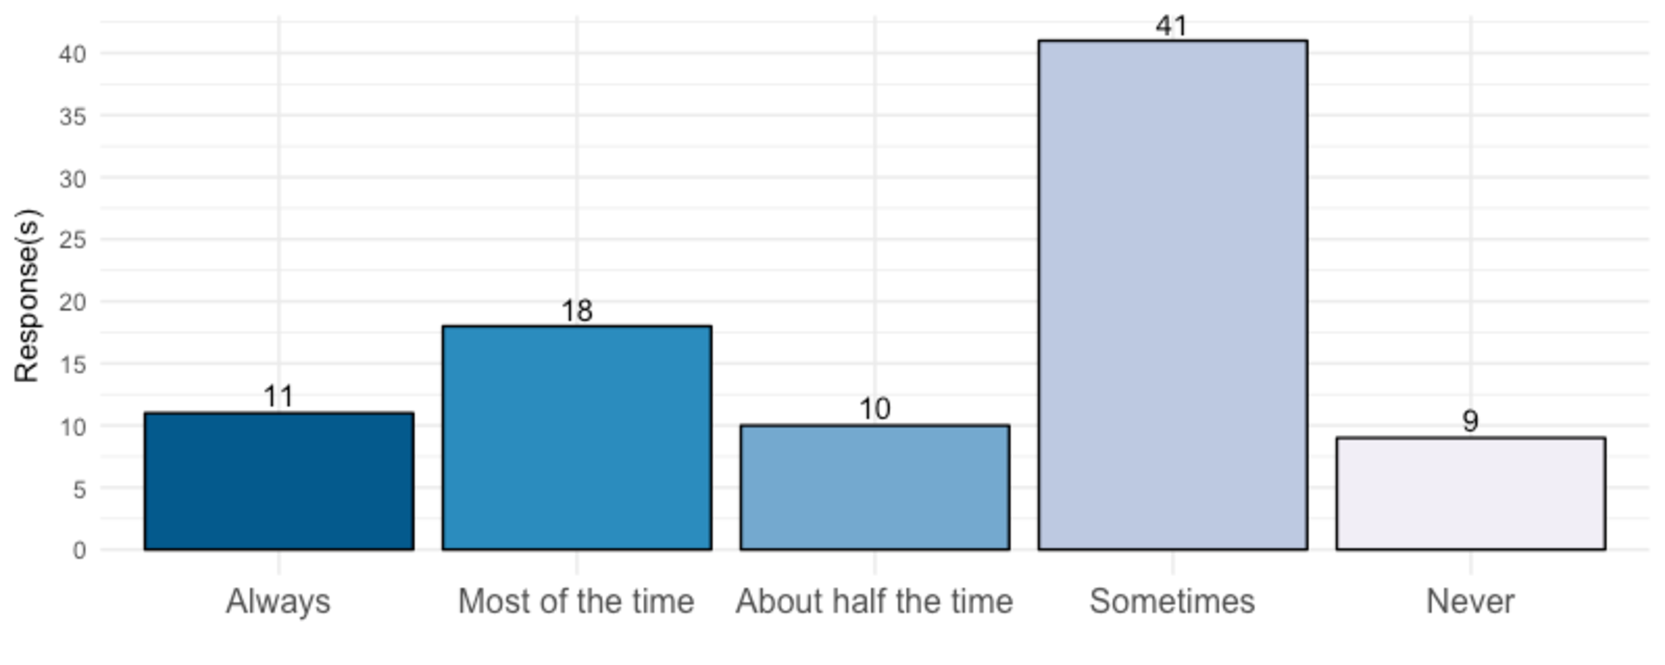
\includegraphics[width=0.98\textwidth,keepaspectratio]{imgs/CodeOwnershipFactor}}
\caption{Degree of Code Ownership as a Factor in Merge Conflict Strategies. Scale: 1 is \textit{Always} and 5 is \textit{Never}. 89 out of 102 respondents (87.26\%) provided a response to this question on the \textit{Processes Survey}~(S1).}
\label{model}
\end{figure}

As an additional question to explore this factor, we asked participants how often \textit{code ownership} factored into their merge conflict resolution strategy.
We found that on average participants indicate that it factors in \textit{about half the time} (mean: 3.21 on a 5-point Likert-type scale).
Only 10.11\% of participants indicated that code ownership \textit{never} factors into their resolution strategy (see Figure~\ref{s1_conflict_urgency}).
\end{comment}

\subsubsection{\textbf{RQ1c}: How do software developers \textbf{evaluate} merge conflict resolutions?}\label{RQ1c}
\vspace*{-0.5\baselineskip}
\begin{center}
\fbox{\parbox{\dimexpr\linewidth-5\fboxsep-2\fboxrule\relax}{\small\centering\raggedleft \textit{``We fail more often because we solve the wrong problem than because we get the wrong solution to the right problem.''\\ -- Russell L. Ackoff}}}%
\end{center}
\vspace*{+0.3\baselineskip}

After implementing a merge conflict resolution, software developers must evaluate whether their resolution has returned the codebase to a clean state.
However, it is unclear what conditions are considered by developers to be the benchmark of a successful merge conflict resolution.

\nsubsection{Success Conditions for Merge Conflict Resolutions}

We examined interview responses to understand which conditions developers use to evaluate their merge conflict resolution.
Developers described six common conditions they considered important in their evaluation.
In the \textit{Processes Survey}~(S1), we asked developers to select all of the six conditions that they would consider for a successful merge conflict resolution.
To allow for additional conditions to surface, we included an open-ended \textit{Other} option.
Only two developers selected that condition, indicating ``performance tests showing similar performance'' and ``client approval.''
We received 324 selections from 89 respondents and present the aggregated results in Table~\ref{conditionsSuccess}.

\begin{table}[!htbp]
\caption{Conditions of Successful Merge Conflict Resolutions from Processes Survey (S1)\textsuperscript{i}}
\label{conditionsSuccess}
\centering
\begin{tabularx}{\textwidth}{@{}lr|*{7}{C}c@{}}
\toprule
	&
	& C1
	& C2
	& C3
	& C4
	& C5
	& C6
	& C7 \\
\midrule
	C1 & All tests pass & \textbf{67} & & & & & & \\
	C2 & Code compiles & 50 & \textbf{67} & & & & & \\
	C3 & Code looks correct & 50 & 54 & \textbf{66} & & & & \\
	C4 & VCS warmings gone & 38 & 42 & 41 & 51 & & & \\
	C5 & Code reviewed & 32 & 31 & 27 & 25 & 38 & & \\
	C6 & Merged to production & 27 & 27 & 27 & 26 & 19 & 33 & \\
	C7 & Other & 2 & 2 & 0 & 0 & 0 & 0 & 2 \\
\bottomrule
    \multicolumn{9}{c}{\noindent\parbox[t]{11.7cm}{\vspace{0.4em}\textsuperscript{i}\hspace{0.2em}\textit{Processes Survey}~(S1) respondents were allowed to select multiple conditions. Each entry represents the number of respondents that selected both of the conditions indicated for the column and row. 68 out of 102 respondents (67\%) selected three or more conditions.}\vspace*{-0.3\baselineskip}} \\
\end{tabularx}
\end{table}

\textit{All tests pass} (C1), \textit{code successfully compiles} (C2), and \textit{code looks correct (i.e. visual test passes)} (C3) were the most commonly selected conditions required for a successful merge resolution.
These results are in line with existing literature showing that testing (C1) can be used for validating program functionality and correctness~\cite{beizer1984software,tian2005software}. %and have been fundamental to development processes such as test-driven development for several years~\cite{beck2003test}.
Similarly, the use of compilers to validate code (C2) as being executable and in good-working order will be familiar to any developer using a compiled programming language.

The use of visual inspection as a measure of successful merge conflict resolutions is surprising, given that \textit{complexity of conflicting lines of code}~(F1) is the highest rate factor for impact on merge conflict difficulty~\cite{mckee2017software}.
Inspecting code requires time and expertise in the area of conflicting code.
The survey respondents that selected \textit{code looks correct (i.e. visual test passes)}~(C3) had a mean of 9.2 years of programming experience, which is only slightly higher than the overall mean of 9.0 years of programming experience.

Looking at the combination of \textit{code looks correct (i.e. visual test passes)}~(C3) with the other conditions, we find that 54 respondents also selected \textit{all tests pass}~(C1) (52.9\%).
As the most common pairing of selected conditions on the \textit{Processes Survey}~(S1), we conclude that although developers rely upon their expertise to visually inspect a merge conflict resolution, they also run the test suite to validate their evaluation.

\nsubsection{Merge Resolution Evaluation Toolsets}

Testing and compilation are used as criteria for determining a successful resolution.
And both require tools with adequate features for developers to make conclusions about the underlying code. 

From the \textit{Exploratory Interviews}, we identified five categories of software development tools that developers mention in relation to merge conflicts.
In the \textit{Processes Survey}~(S1), we asked the developers to identify the tools they use when evaluating a merge conflict resolution.
We received 204 selections from 89 respondents.
The aggregated results are presented in Table~\ref{resolution-evaluation-tools}, ranked according to the percentage of respondents that selected each toolset.

\begin{table}[!htbp]
\renewcommand{\arraystretch}{1.2}
\caption{Merge Resolution Evaluation Toolsets from Processes Survey (S1)}
\label{resolution-evaluation-tools}
\centering
\begin{tabularx}{\textwidth}{>{\rowmac}l | >{\rowmac}c | >{\rowmac}r <{\clearrow}}
\toprule
  \parnoteclear % tabularx will otherwise add each note thrice
  Description & \# Selections\parnote{\textit{Processes Survey}~(S1) respondents were allowed to select multiple toolsets. 64 out of 89 respondents (71.91\%) selected multiple toolsets.\vspace*{-0.3\baselineskip}} & Percentage (\%)\textsuperscript{i} \\
\midrule
  Version Control Systems (e.g. Git, Subversion, CVS) & 82 & 92.14\% \\
  Continuous Integration (e.g. TravisCI, Jenkins, TFS) & 62 & 69.66\% \\
  Program Analysis Tools (e.g. Coverity, CodeSonar) & 26 & 29.21\% \\
  DevOps Tools (e.g. Nagios, Monit, Kabana) & 17 & 19.10\% \\
  Release Management Tools (e.g. Chef, Puppet, Salt) & 9 & 10.11\% \\
  Other Tools & 8 & 8.99\% \\
\bottomrule
\end{tabularx}
\parnotes
\end{table}
\vspace{0.8em}

By far, the most selected tools were \textit{version control systems} (VCS) and \textit{continuous integration} (CI) platforms, with 82 (92.14\%) and 62 (69.66\%), respectively.
The mean for all other tool categories was 15 selections (16.85\%), and represents a combined 29.4\% of response selections.

The use of version control systems to determine whether a resolution was successful aligns with \textit{VCS warnings are gone} (C3) being the fourth most selected success condition (see Table~\ref{conditionsSuccess}).
Also, continuous integration is dependent on code being compilable (C2), and tests being written and maintained (C1).
However, the availability of tools for evaluating merge conflict resolutions might constrain the conditions that developers are willing to consider.
Further research is needed to determine whether there is a causal relationship between these dimensions, and whether more effective metrics could be supported by merge conflict toolsets.

\nsubsection{Backup Strategies}

Merge conflict resolutions are not always successful.
When they fail, developers must alter their patch and potentially switch strategies in order to successfully resolve the conflict.

To understand the prevalence of failed conflict resolutions, we asked \textit{Processes Survey}~(S1) participants to indicate the frequency in which their first attempt at resolving a merge conflict fails.
Figure~\ref{fig:first-attempt-failure} illustrates the resulting distribution on a 5-point Likert scale, where 1 is \textit{very frequently} and 5 is \textit{very infrequently,} the mean response was 3.49 ($std. dev.=1.11$, $variance=1.24$).
This corresponds to \textit{somewhat infrequently} being both the average response and the most common response ($median=4$), which suggests that first attempts typically succeed.
However, this also shows that 78.7\% of participants (70 out of 89) occasionally fail at their first attempt and must make additional attempts to resolve a merge conflict.

\begin{figure}
	\centering
	\fbox{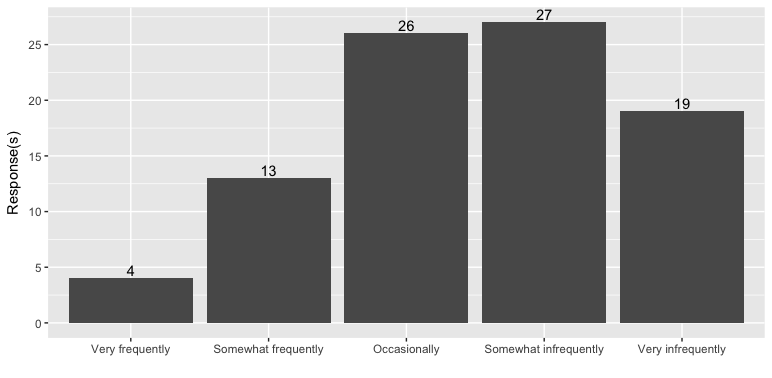
\includegraphics[width=0.95\textwidth,keepaspectratio]{FirstAttemptFailure}}
	\caption{Frequency of Failures in First Attempts at Merge Conflict Resolution. Scale: 1 is \textit{Very frequently} and 5 is \textit{very infrequently}. 89 out of 102 respondents (87.26\%) provided a response to this question in the \textit{Processes Survey}~(S1).\vspace*{-0.3\baselineskip}}
	\label{fig:first-attempt-failure}
\end{figure}

Furthermore, we asked survey participants to describe their backup strategies when their first attempt at resolving a merge conflict fails.
We received 75 responses and the aggregate results are presented in Table~\ref{backup-strategies}, ranked according to the percentage of respondents that described using each backup strategy.

Developers' backup strategies include \textit{take it offline} (B1), \textit{collaborating} (B2), \textit{try again} (B3), \textit{redoing changes} (B4), and \textit{no backup strategy} (B5).
Since \textit{no backup strategy} (B5) is not a strategy in and of itself, we focus on strategies B1--B4 instead.

%TODO I feel that this discussion should be moved to the discussion section... -Caius
The \textit{take it offline} (B1) strategy involves moving conflicting code away from shared branches or code repositories, and working locally to resolve the conflict without disrupting other developers.
The antithesis of this strategy is \textit{collaborating} (S2), where developers seek out other developers that are more knowledgeable about the area of conflicting code.
The B1 and B2 strategies contrast each other, and show that developers reserve more costly strategies (in terms of time, effort, and coordination) as backups to their primary resolution strategies.

Additionally, we find that developers also simply \textit{try again} (B3) to merge the same code together and hope that their tools are able to succeed with a second attempt.
Developers also resort to \textit{redoing changes} (B4), by way of reverting and manually recreating the changes found in conflicting commits when their initial attempt failed.
The B3 and B4 strategies appear to cement the extremes of the cost spectrum of backup strategies for resolving merge conflicts.
Simply retrying the same merge (B3) requires very little additional work, whereas the process of redoing changes (B4) is a duplication of previous efforts and is therefore costly on developer's time.

\begin{table}[!htbp]
\renewcommand{\arraystretch}{1.2}
\caption{Backup Strategies for Resolving Merge Conflicts from Processes Survey (S1)}
\label{backup-strategies}
\centering
\begin{tabularx}{\textwidth}{c|l|c|r}
\toprule
  \parnoteclear % tabularx will otherwise add each note thrice
  Strategy & Description & \# Participants\parnote{75 out of 102 respondents (73.53\%) provided a description of their backup strategy.\vspace*{-0.3\baselineskip}} & Percentage (\%)\textsuperscript{i} \\
\midrule
  B1 & Take it offline & 19 & 25.33\% \\
  B2 & Collaborating & 17 & 22.67\% \\
  B3 & Try again & 15 & 20.00\% \\
  B4 & Redoing changes & 14 & 18.67\% \\
  B5 & No backup strategy\hspace{2.0cm} & 10 & 13.33\% \\
\bottomrule
\end{tabularx}
\parnotes
\end{table}
\vspace{0.8em}